\documentclass[12pt,twoside]{article}
\usepackage{jmlda}
%автомат

\title
    [HG-LBP дескриптор на основе гистограмм градиентов для детектирования пешеходов] % Краткое название; не нужно, если полное название влезает в~колонтитул
	{Метод построения HG-LBP дескриптора на основе гистограмм градиентов для детектирования пешеходов}
\author
    [Разумов~И.\,О, Прошутинский~Д.\,А, Гнеушев~А.\,Н.] % список авторов для колонтитула; не нужен, если основной список влезает в колонтитул
    {Разумов$^1$~И.\,О, Прошутинский$^1$~Д.\,А, Гнеушев$^{1,2}$~А.\,Н.} % основной список авторов, выводимый в оглавление
    [Разумов$^1$~И.\,О, Прошутинский$^1$~Д.\,А, Гнеушев$^{1,2}$~А.\,Н.] % список авторов, выводимый в заголовок; не нужен, если он не отличается от основного
\thanks
    {Работа выполнена при финансовой поддержке РФФИ, проект \No\,00-00-00000.
   Научный руководитель: Матвеев~И.\,А. 
   Задачу поставил и консультировал: Гнеушев~А.\,Н.}
\email
    {razzumoff@gmail.com, gneushev@ccas.ru, dmitriy.proshutinskiy@phystech.edu}
\organization
    {$^1$Московский физико-технический институт, Россия, г. Долгопрудный, Институтский пер., 9\par
     $^2$ФИЦ <<Информатика и управление>> РАН, Россия, г. Москва, ул. Вавилова, 44/2}
\abstract
   {Рассматривается подход обобщения алгоритма LBP (Local Binary Patterns) для детектирования пешеходов 
   на изображении на основе учета вклада каждого LPB-кода в пространственную гистограмму дескриптора. Обычный LPB дескриптор включает гистограмму только количества вхождений LBP-кода в локальной области изображения и не учитывает степень выраженности каждого LPB-кода. В статье предлагается использовать вес каждого LBP-кода при построении локальной гистограммы дескриптора. Рассматриваются два варианта оценки веса LPB: на основе модуля градиента и на основе суммы модулей производных по восьми направлениям в точке подсчета LBP-кода для формирования нового дескриптора HG-LPB (Histogram Gradient LBP). Учет локальной выраженности LPB-кода позволяет учитывать больше информации о локальных особенностях изображения объекта в HG-LPB дескрипторе и улучшить качество работы детектора. В статье представлены результаты сравнения работы базовых алгоритмов LPB, HOG-LBP и предлагаемых обобщений HG-LPB на базе изображений пешеходов INRIA.
\bigskip
\textbf{Ключевые слова}: \emph {LPB, HOG, гистограмм ориентированных градиентов, Локальные бинарные шаблоны, детектирование пешехода}.}
\titleEng
    {HG-LBP descriptor based on gradient histograms for pedestrian detection}
\authorEng
    {Razumov$^1$~I.\,O., Proshutinskii$^1$~D.\,A., Gneushev$^{1,2}$~A.\,N.}
\organizationEng
    {$^1$Moscow Institute of Physics and Technology, 9 Institutskiy per., Dolgoprudny, Moscow, Russia\par
	$^2$Federal Research Center ``Computer Science and Control'' of RAS, 44/2 Vavilova Str., Moscow, Russia}
\abstractEng
    {In this work we offer the approach is considered to generalize the LBP (Local Binary Patterns) algorithm for detecting pedestrians in an image based on taking into account the contribution of each LPB code to the spatial histogram of the descriptor. A regular LPB descriptor includes a histogram of only the number of occurrences of the LBP code in the local image area and does not take into account the severity of each LPB code. The article proposes to use the weight of each LBP code when constructing a local histogram of the descriptor. Two options for estimating the weight of the LPB are considered: based on the modulus of the gradient and on the basis of the sum of the modules of the derivatives in eight directions at the LBP code counting point to form the Histogram Gradient LBP. Taking into account the local manifestation of the LPB-code allows you to take into account more information about the local features of the image of the object in the HG-LPB descriptor and improve the quality of the detector. The article presents the results of a comparison of the work of the basic LPB, HOG-LBP algorithms and the proposed HG-LPB generalizations based on the images of INRIA pedestrians.

    \bigskip
    \textbf{Keywords}: \emph{LPB, HOG, Histograms of Oriented Gradients, Local Binary Patterns, pedestrian detection}.}
\begin{document}
\maketitle
%\linenumbers
\section{Введение}
Автоматическое детектирование и распознавание объектов на изображениях является одной из основных задач компьютерного зрения. 
Задача локализации человека на видеоизображениях широко востребована в таких областях, как мониторинг и анализ дорожных ситуаций, обнаружение дорожно-транспортных происшествий, контроль за соблюдением правил дорожного движения, системы безопасности и следящие системы, беспилотные автомобили, робототехника, системы помощи водителю.

Основные сложности обнаружения человека на изображении связаны с несколькими причинами: изменение структуры изображения вследствие движения человека, неравномерная освещенность изображения, большая вариабельность изображений человека из-за разных ракурсов (поз, размеров, углов поворота), частичные перекрытия фигуры человека другими объектами.

Как правило, задача детектирования объекта разделяется на две подзадачи: выделение характерных свойств изображения объекта и бинарная классификация. Характерные свойства изображения объекта - это набор признаков, приближенно описывающий интересующий объект. Выбранный набор признаков является важнейшим фактором, влияющим на качество классификации и ее устойчивость. Чем лучше признаки обладают разделительной способностью, тем проще устроено признаковое пространство, и работа классификатора наиболее эффективна. 

Признаки можно разбить на два класса: локальные и интегральные. Преимуществом локальных признаков является их универсальность, инвариантность по отношению к неравномерным изменениям яркости и освещённости, но они не уникальны. В тоже время интегральные признаки, характеризующие изображение объекта в целом, не устойчивы к изменению структуры объекта и сложным условиям освещения. Существует комбинированный подход - использование локальных признаков в качестве элементов интегрального описания, когда искомый объект моделируется набором областей, каждая из которых характеризуется своим набором признаков – локальным текстурным дескриптором. Совокупность таких дескрипторов характеризует объект в целом.

Вид локальных признаков определяется характерной структурой объекта на изображении. Изображение человека может быть представлено совокупностью контуров, силуэтов частей тела, которые являются контурными признаками и представляются на изображении как максимальные перепады значений яркости \cite{Gneushev03}. Для описания локальной контурной структуры изображения пешехода широко применяются подходы основанные на Гистограмме Ориентаций Градиентов (НОG)~\cite{dalaltriggs2005}, на Локальных Бинарных Шаблонах~\cite{dalaltriggs2005} и сверточных нейронных сетях (CNN).

Использование сверточных нейронных сетей являются довольно эффективным подходом для одновременного выделения множества локальных признаков и их классификации. В CNN процедура выделения признаков осуществляется в начальных слоях, структура признаков формируется автоматически в процессе его обучения и определяется моделью и архитектурой сети. Чем больше признаков необходимо использовать для характеристики целевых объектов, тем больше параметров требуется для задания модели сети, тем она вычислительно сложнее и требует больше вычислительных ресурсов и объема обучающей выборки изображений. Это связано с тем, что в CNN признаковая модель объекта формируется на основе только той информации, которая содержится в обучающей базе и общих регуляризационных ограничениях. Однако использование априорной, более детальной экспертной информации о характере конкретного класса объектов на изображении для построения пространства признаков и получения дескрипторов позволяет существенно уменьшить объем вычислений при той же точности работы системы. Таким образом, использование дескрипторов, построенных на методах HOG и LPB, остаются актуальными для вычислительно слабых платформ.

Дескрипторы HOG и LBP обладают рядом недостатков, каждый из ни учитывает не всю полезную информацию о структуре изображения. Одним из подходов для усложнения пространства признаков является объединение этих дескрипторов в один HOG-LPB~\cite{Wang09}. Однако простое объединение не всегда эффективно, есть подходы модификации самих дескрипторов с использованием полезных свойств друг друга. Так, в работе~\cite{Samsonov17} предлагается обобщить HOG дескприптор в HAH-AR и использовать информацио о положении контурных признаков. Обычный LPB дескриптор~\cite{Ojala02} включает гистограмму только количества вхождений LBP-кода в локальной области изображения и не учитывает степень выраженности каждого LPB-кода, однако подобная выраженность контурных признаков используется в гистограммах HOG дескриптора.

В статье предлагается подход обобщения LPB дескриптора на основе использования веса каждого LBP-кода при построении локальной гистограммы дескриптора. Предлагается два варианта оценки веса LPB: на основе модуля градиента и на основе суммы модулей производных по восьми направлениям в точке подсчета LBP-кода для формирования нового дескриптора HG-LPB (Histogram Gradient LBP). Учет локальной выраженности LPB-кода позволяет учитывать больше информации о локальных особенностях изображения объекта в HG-LPB дескрипторе и улучшить качество работы детектора.

\section{Существующие подходы}
\subsection{Используемые модели}
\textbf{Local Binary Pattern (LBP)}: LBP был представлен в 1994 году [8]. Однако, модель спектра текстуры LBP была предложена еще ранее в 1990 году [9]. Оператор LBP был применен во многих областях после исследований Ojala и Pietikäinen в области подхода с несколькими разрешениями в 2002 году [10], включая идентификацию текста [11] и распознавание лиц [5]. Wang объединил LBP с дескриптором гистограммы направленных градиентов (HOG) для повышения эффективности обнаружения в [12]. К данной статье мы ещё вернёмся. Классический оператор LBP должен следовать определенному алгоритму; Эти действия суммированы на рис. 1 [7]. Есть ряд попыток улучшить метод LBP. Одна недавняя версия находит значения интенсивности точек в круговой окрестности, рассматривая значения, которые имеют маленькие круговые окрестности вокруг центрального пикселя [13].

\textbf{Histogram of Oriented Gradients (HOG)}: HOG -- дескриптор, основаный на подсчете количества направлений градиента в локальных областях изображения. Традиционный HOG делит изображение на разные области, именнуемые ячейками, и вычисляет гистограммы направлений градиентов или направлений краев для пикселей [13]. HOG широко применяется в областях распознавания объектов как распознавание лиц [14]. Процесс вычисления HOG объясняется на рис. 2 [15].

\textbf{Вектор опорных векторов (SVM)}: SVM - это алгоритм обучения с учителем, разработанный для бинарных задач классификации с возможным расширением до многоклассовых задач [23]. Кортес и Вапник впервые представили SVM в 1995 году, основная идея которого заключалась в том, что каждый объект данных представляется вектором в k-мероном пространстве и пренадлежит одному из двух классов. После ищется такая гиперплоскость размерности (p-1), что расстояние до ближайших к гиперплоскости точек из разных классов максимально. Такая гиперплоскость называется оптимальной. Позже Кортес и Вапник ввели понятие мягких границ, суть которых заколючается в возможности классификатора допускать ошибки в случае линейной неразделимости выборки, чтобы в конечном итоге всё таки построить разделяющую гиперплоскость[24]. Некоторыми преимуществами SVM являются обобщение бинарных и регрессионных форм и упрощение обозначений [23]. В SVM можно использовать одно из несколько ядер: полиномиальное, линейное, радиальная базисная функция Гаусса(RBF) [25], [26] и т.д.


% обзор литературы
\subsection{Работа с датасетом изображений}
В данной работе в качестве набора изображений людей использовался датасет INRIA\cite{inria}. Данный набор данных был собран в рамках исследовательской работы по обнаружению вертикально расположенных людей на изображениях и видео\cite{dalaltriggs2005}. Набор данных делится на 2 формата: (а) исходные изображения с соответствующими файлами аннотаций и (b) положительные изображения в нормализованном формате 64x128 пикселей (как используется в документе CVPR) с исходными отрицательными изображениями.

Мы использовали нормализованные данные, которые распределены в две папки: тест и обучение. Обе папки имеют две подпапки: (a) «pos» (нормализованные положительные тренировочные или тестовые изображения, центрированные на человеке с их лево-правыми отражениями), (b) «neg» (содержащие оригинальные отрицательные тренировочные или тестовые изображения). Положительные изображения в папке обучения имеют размер 96x160 пикселей (с полями в 16 пикселей вокруг каждой стороны), а положительные изображения в папке теста имеют размер 70x134 пикселей (с полями 3 пикселя вокруг каждой стороны). Это было сделано, чтобы избежать граничных условий (таким образом, чтобы избежать какого-либо конкретного смещения в классификаторе). В обеих папках используйте центрированное окно 64x128 пикселей для исходной задачи обнаружения.

Для создания отрицательных обучающих окон из нормализованных изображений фиксированный набор из 12180 окон (10 окон на негативное изображение) выбирается случайным образом из 1218 отрицательных обучающих фотографий, обеспечивающих исходный отрицательный обучающий набор.

\subsection{Референтые работы}
Близкой к теме данной работы является статья <<An HOG-LBP Human Detector with Partial Occlusion Handling>> Xiaoyu Wang \cite{Wang09}. В данной статье комбинируется гистограммы направленных градиентов (HOG) и локальные бинарные шаблоны (LBP) для получения набора признаков. Это делается для улучшенной точности определения человека на изображении даже в ситуации с частично закрытой фигурой человека. Процедура обнаружения человека, основанная на функции HOG-LBP, показана на \ref{fg:Wang1}. Похожую схему мы используем в нашей работе. 

\begin{figure}[H]
	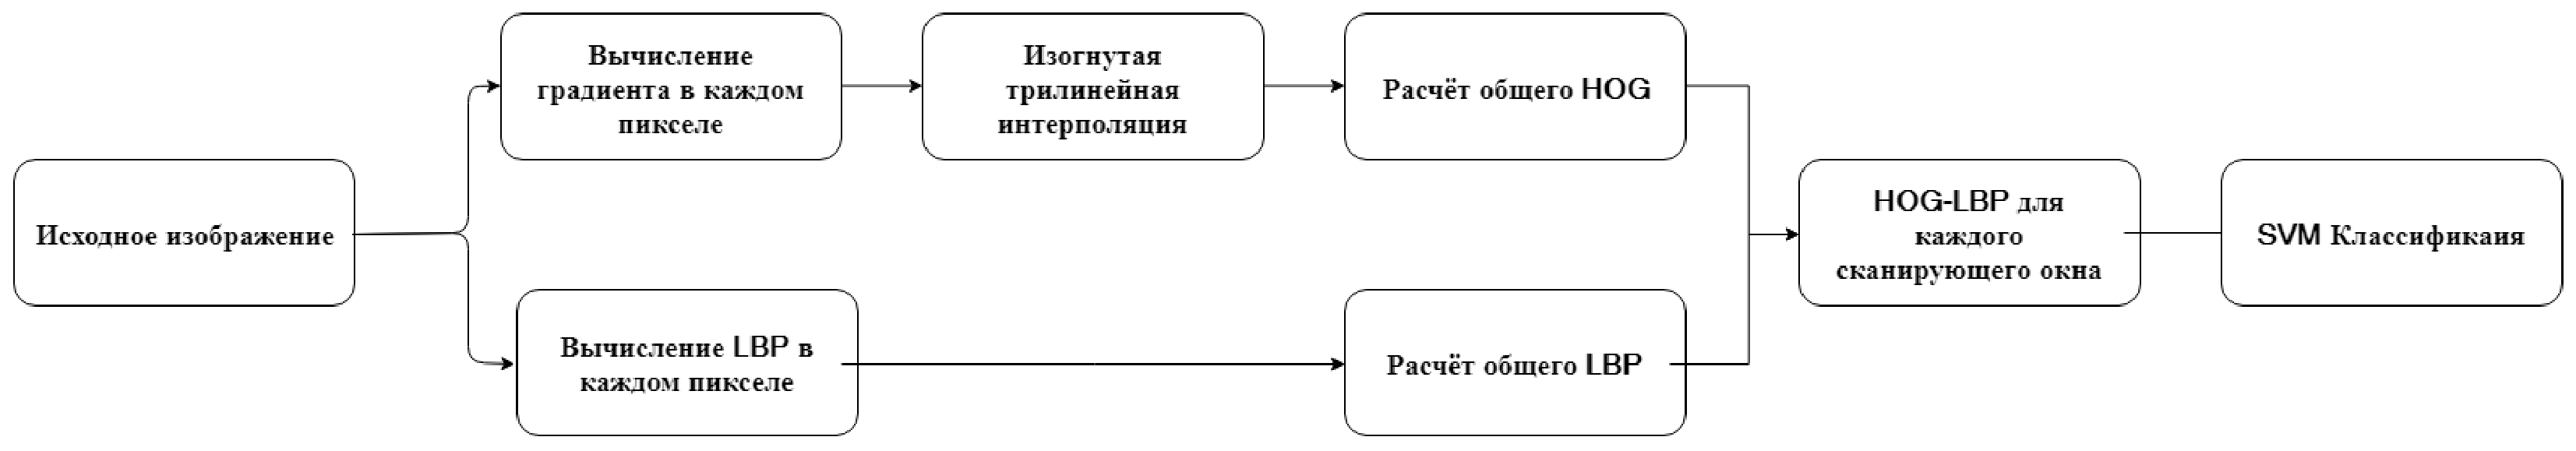
\includegraphics[width=1\textwidth]{Graph}
	\caption{Подпись должна размещаться под рисунком. }
	\label{fg:Wang1}
\end{figure}




\section{Постановка задачи}
Рассмотрим структуру интегрального вектора признаков $\vec{g}(f) = (g_{1},\dots , g_{n})^{\mathrm{T}}$ HOG дескриптора \cite{dalaltriggs2005} из признакового пространства $G$ для входного изображения $f$, где $n$~--- размерность пространства признаков. В соответствии со схемой
HOG, изображение $f(x,y)$, где $x$, $y$~--– координаты точки изображения размером $X\times Y$, разбивается на смежные области~--– квадратные ячейки размером $K\times K$ пикселей, $I=X/K$ ячеек по горизонтали и $J=Y/K$ ячеек по вертикали. 
В каждой ячейке $(i,j)$, где $i$, $j$~--- индексы ячейки по вертикали 	и горизонтали соответственно, выделяются локальные признаки, которые определяются дескриптором ячейки~--- вектором $\vec{u}_{i,j} = (u_1, \dots , u_l)^{\mathrm{T}}$, где $l$~---	размерность вектора. Четыре смежные ячейки объединяются в пересекающиеся блоки. Таким образом, каждый блок содержит $4K \times 4K$ пикселей и имеет общие ячейки с соседними блоками. Дескриптор блока определяется объединением дескрипторов собственных ячеек, вектором $\vec{v}_{i,j} = \vec{u}_{i,j}\cup\vec{u}_{i+1,j}\cup\vec{u}_{i,j+1}
	\cup\vec{u}_{i+1,j+1},$ где $i$,$j$~--- индексы блока.
	Общее количество блоков~--- $(I-1)(J-1)$. Под операцией
	объединения $\cup$ двух векторов $\vec{u}_{1}$ и $\vec{u}_{2}$
	c размерностью $l_{1}$ и $l_{2}$ соответственно будем понимать результирующий вектор из пространства размерности $l_{1}+l_{2}$, первые $l_{1}$ компонент которого являются компонентами вектора первого аргумента, последние $l_{2}$ ~--- компонентами вектора второго аргумента.
	
	 Дескриптор блока нормируется с помощью одной из двух норм:
		 $L_2$ нормы
\begin{equation*}
	\vec{\tilde{v}} = N_{L_{2}}(\vec{v}) =  \frac{\vec{v}}{\sqrt{\Vert \vec{v} \Vert_{2}^{2} + \epsilon^{2}}}
	\label{eq:L2}
\end{equation*}
либо $L_2$--hys нормы \cite{dalaltriggs2005}
\begin{equation*}
	\vec{\tilde{v}} = N_{L_{2}-\mathrm{hys}}(\vec{v}) =  N_{L_{2}}
	\left(\min(N_{L_{2}}(\vec{v}),h)\right),
	\label{eq:L2-hys}
\end{equation*}
где операция $\min$ применяется покомпонентно к вектору первого
аргумента; $h$~--- пороговое значение, которое используется для
ограничения значений компонент вектора в~операции $\min$. В данной работе, как и в работе \cite{dalaltriggs2005}, в качестве порогового значения используется $h=0{,}2$.


Интегральный дескриптор определяется объединением всех
блочных дескрипторов, т.\,е.\ вектором
\begin{equation}
\vec {g}=\bigcup_j^{J-1}{\bigcup_i^{I-1}{\vec{\tilde{v}}_{i,j}}}\,.
\end{equation}
Интегральные дескрипторы $\vec{g}$ множества изображений формируют
признаковое пространство $G$. 

В работе ставится задача преобразования признакового векторного пространства $G$ в трехмерное тензорное пространство с размерностью ${2(I-1)}\times{2(J-1})\times{l}$, восстанавливающее пространственную смежность дескрипторов ячеек $\vec{u}$ из блоков $\vec{v}$ вектора $\vec{g}$. Используя тензорное представление вектора $\vec{g}$ реализовать сверточную нейронную сети одной из известных архитектур для решения задачи разбиения этого пространства
на два непересекающихся класса: первый характеризует пешеходов; второй~--- фон, не содержащий пешехода. 

Множество весов и параметров нейросетевого классификатора находятся из процедуры обучения по специально подготовленной 
обучающей выборке из базы изображений INRIA, CityScapes \cite{inria} содержащие два подмножества изображений: 
с~положительными примерами, содержащими пешеходов, и отрицательными примерами, содержащими фон.

	Критерием качества классификации  на специально
	подготовленной тестовой выборке из базы изображений INRIA \cite{inria} и CityScapes
	будем считать отношение $\mathrm{MR} = \mathrm{FN}/(\mathrm{TP}+\mathrm{FN})$~---
	доля неверно отвергнутых классификатором изображений ($\mathrm{Miss\ Rate}$),
	к $\mathrm{FPPW} = \mathrm{FP}/(\mathrm{TN}+\mathrm{FP})$~---
	доля неверно принятых изображений ($\mathrm{False\ Positive\ Per\
	Window}$), где $\mathrm{FN}$~--- количество неверно отвергнутых
	классификатором положительных примеров; $\mathrm{TP}$~---
	количество верно классифицированных положительных примеров;
	$\mathrm{TN}$~--- количество верно классифицированных отрицательных
	примеров; $\mathrm{FP}$~--- количество неверно классифицированных отрицательных примеров.


\section{Тензорное представление HOG дескриптора для CNN}


\section{Результаты вычислительных экспериментов}

\section{Заключение}
Желательно, чтобы этот раздел был, причём он не~должен дословно повторять аннотацию.
Обычно здесь отмечают,
каких результатов удалось добиться,
какие проблемы остались открытыми.

\bigskip
%\newpage
\maketitleSecondary
%\English

\bibliographystyle{unsrt}
\bibliography{Project30}

\begin{thebibliography}{99}
\bibitem{Gneushev03}
Gneushev, A.\,N., and A.\,B.~Murynin.	
2003. Adaptive gradient method for extracting contour features of
objects in images of real-world scenes.
\BibJournal{J.~Comput. Sys. Sci. Int.} 42(6):973--980.

\bibitem{Gneushev07}
Гнеушев А.Н. Построение и оптимизация текстурно-геометрической модели изображения лица в пространстве базисных функций Габора. // Известия Академии Наук. Теория и системы управления. – 2007. – № 3. – c. 85-96.

\bibitem{Samsonov17}
Samsonov N.\,A., Gneushev, A.\,N.	
2017. Textural descriptor in the Hough accumulator space of the gradient field for detecting pedestrians.
\BibJournal{Machine Learning and Data Analysis} 3(3):203--215.

\bibitem{dalaltriggs2005}
Dalal,~N., and B.~Triggs. 2005.
 Histograms of oriented gradients for
human detection. \BibJournal{IEEE CVPR}. San Diego, CA.

\bibitem{Wang09}
Wang,~X., Han~X., Yan,~S. 2009.
 An HOG-LBP Human Detector with Partial Occlusion Handling. \BibJournal{ICCV}.

\bibitem{Ojala02}
Ojala,~N., and M.~Pietikainen 2002.
 Multiresolution Gray-Scale and Rotation Invariant Texture Classification with Local Binary Patterns, IEEE Trans on Pattern Analysis and Machine Intelligence.
\BibJournal{IEEE Trans on Pattern Analysis and Machine Intelligence} 7(24).
 
\bibitem{dpm}
	{Felzenszwalb,~P.\,F., B.\,R.~Girshick, D.~McAllester,
	and D.~Ramanan}. 2010.
	Object detection with discriminatively trained part based models.
\BibJournal{IEEE T.~Patt. Anal.} 32(9):1627--1645.

\bibitem{sunwatanada2015}
	{Sun,~D., and J.~Watanada}, 2015.
	Detecting pedestrians and vehicles in traffic scene based on
	boosted HOG features and SVM.
\BibJournal{IEEE 9th  Symposium (International)
on Intelligent Signal Processing}.

\bibitem{inria}
	INRIA Person Dataset.
	Avalaible at: {\sf http://pascal.inrialpes.fr/data/human/}
	(accessed June~4, 2017).

\bibitem{opencv}
	Open Source Computer Vision Library.
	Avalaible at: {\sf http://opencv.org/releases.html}
	(accessed May 16, 2017).
	
\bibitem{Vorontsov}
	Vorontsov, K.\,V. 2007. Lectures on support vector machine.
	{\sf http://www.ccas.ru/voron/download/\linebreak SVM.pdf}
	(accessed June~25, 2017).
	

\end{thebibliography}

% Решение Программного Комитета:
%\ACCEPTNOTE
%\AMENDNOTE
%\REJECTNOTE
\end{document}
